\documentclass[a4]{article}

\usepackage[left=2cm,right=2cm,top=2cm,bottom=2cm]{geometry} 

\usepackage[utf8]{inputenc}   % otra alternativa para los caracteres acentuados y la "ñ"
\usepackage[           spanish % para poder usar el español
                      ,es-tabla % para los captions de las tablas
                       ]{babel}   
\decimalpoint %para usar el punto decimal en vez de coma para los números con decimales

%\usepackage{beton}
%\usepackage[T1]{fontenc}

\usepackage{parskip}
\usepackage{xcolor}

\usepackage{caption}

\usepackage{enumerate} % paquete para poder personalizar fácilmente la apariencia de las listas enumerativas

\usepackage{graphicx} % figuras
\usepackage{subfigure} % subfiguras

\usepackage{amsfonts}
\usepackage{amsmath}

\definecolor{gris}{RGB}{220,220,220}
	
\usepackage{float} % para controlar la situación de los entornos flotantes

\restylefloat{figure}
\restylefloat{table} 
\setlength{\parindent}{0mm}


\usepackage[bookmarks=true,
            bookmarksnumbered=false, % true means bookmarks in 
                                     % left window are numbered
            bookmarksopen=false,     % true means only level 1
                                     % are displayed.
            colorlinks=true,
            allcolors=blue,
            urlcolor=cyan]{hyperref}
\definecolor{webblue}{rgb}{0, 0, 0.5}  % less intense blue


\title{Aprendizaje Automático: Proyecto Final \\ Devanagari Handwritten Characters}

\author{David Cabezas Berrido y Patricia Córdoba Hidalgo}

\date{}

\begin{document}

\maketitle
\tableofcontents

\newpage

\section{Problema}

El problema a resolver consiste en clasificar caracteres de la
escritura Devanagari. Nuestros datos son imágenes de estos símbolos
escritos a mano, cada uno de ellos con una etiqueta especificando el
símbolo que representa la imagen.

Inicialemente, nuestro espacio de características $\mathcal{X}$ está
formado por imágenes de $32 \times 32$ píxeles cada una, con un marco
de $2$ píxeles por cada uno de los $4$ lados. El conjunto de
etiquetas, $Y$ son los $46$ caracteres que consideramos, $36$ letras y
$10$ dígitos (del $0$ a $9$). La función objetivo $f$ que buscamos es
aquella que a una cuadrícula de píxeles representando un símbolo
Devanagari manuscrito le haga corresponder la clase del símbolo
correspondiente.

\section{Dataset. Conjuntos de train y test}

El conjunto de datos de los que disponemos \\
\href{https://archive.ics.uci.edu/ml/datasets/Devanagari+Handwritten+Character+Dataset}{https://archive.ics.uci.edu/ml/datasets/Devanagari+Handwritten+Character+Dataset}
consta de 92000 instancias (imágenes etiquetadas), 2000 de cada una de
las 46 clases. Los datos vienen divididos en train: 78200 instancias
(85\%), 1700 por clase; y test: 13800 instancias (15\%), 300 por
clase.

Existen algunos artículos y proyectos relativos a este dataset, por lo
que mantener esta división entre train y test nos permitirá
comparar los resultados que logren nuestros modelos y procesamiento
con los resultados de otros diseñados por terceros.
También sabemos que no existen datos perdidos y las clases están
perfectamente balanceadas.

En la descripción del dataset se informa de que estos datos proceden
de documentos escritos, pero desconocemos su procedencia y sus
autores. En problemas de reconocimiento de símbolos manuscritos existe
la dificultad de que un modelo aprenda a reconocer símbolos de un
único autor o un conjunto de autores, lo que conlleva sobreajuste y a
estimaciones por validación poco fiables, ya que la muestra de
entrenamiento no termina de ser representativa y el modelo se adapta a
ese sesgo. En nuestro caso, desconocemos si los datos de train y test
corresponden a símbolos trazados por distintas personas o no, con lo
que tenemos otra razón más para respetar la partición de conjuntos de
train y test existente.

Extraemos un conjunto de validación del 30\% de los datos de
entrenamiento para consultar la eficacia práctica de ciertas
decisiones que tomamos durante el preprocesamiento, así como para
estimar los hiperparámetros usados en cada modelo. Esto nos deja con
54740 (70\%) datos para entrenar cada alternativa y 23460 datos para
validar. Debido a la abundancia de datos, podemos esperar que los
scores obtenidos al validar sean representativos de la bondad real de
un modelo o procesamiento, así que decidimos no usar validación
cruzada, ya que es computacionalmente muy costosa y el ajuste de los
modelos es lento debido a la cantidad de datos.

Para ello usamos la función \texttt{train\_test\_split} de
\textit{sklearn} e indicamos mediante la opción \texttt{stratify} que
queremos preservar la proporción de elementos de cada clase en cada
uno de los conjuntos, de forma que sigan perfectamente balanceadas.

\subsection{Formato de los datos}

En el fichero \texttt{png\_to\_np.py}, guardamos las imágenes,
originalmente en formato \texttt{png}, como array. Para ello leemos
cada imagen como array de escala de grises usando la función
\texttt{imread} de \textit{matplotlib} y eliminamos los dos píxeles de
marco por cada lado, quedándonos con matrices de $28 \times 28$ de
valores flotantes entre $0$ y $1$ representando la intensidad de gris
en cada pixel. El resultado es guardado en disco, lo hacemos con la
función \texttt{saveGrey}, que usa la función
\texttt{savez\_compressed} de \textit{numpy} para almacenarlo en
formato \texttt{npz}.

Este fichero solo se ejecuta una vez para cambiar el formato de los
datos. Tras esto, podemos usar los datos guardados en disco para las
sucesivas ejecuciones del código. Proporcionamos los datos ya
transformados, aunque en el fichero \texttt{main.py} se puede alterar
la variable \texttt{PNG\_TO\_NP} para ejecutar el script que carga las
imágenes y almacena estos datos en disco.

\section{Preprocesamiento}

% Comentar justificaciones: RF con parámetros por defecto. WIDTH y
% BLOCK_REDUCE

% ¿Vale la pena matriz de Pearson?

% Quizá dos subsecciones y desarrollar y justificar más cada función

Preprocesamos los datos usando las funciones implementadas en el
fichero \texttt{preprocessing.py}. El preprocesamiento se realiza
imagen a imagen, siendo el resultado sólo dependiente de la propia
imagen y por tanto paralelizable. Esta independencia hace que sea
indiferente extraer los datos para validación antes o después del
preprocesamiento. Para cada imagen realizamos dos operaciones:

\subsection{Centrado y reescalado}

Esta operación la realiza la función \texttt{centerAndResize}. Ante
una imagen, calculamos un umbral con la ayuda del \href{https://en.wikipedia.org/wiki/Otsu%27s_method}{método de Otsu}
  para
\href{https://en.wikipedia.org/wiki/Thresholding_(image_processing)}{thresholding} (usando la función \texttt{threshold\_otsu} de la librería \textit{skimage}). 

Para calcular la caja englobante del carácter, usamos el
\href{https://en.wikipedia.org/wiki/Closing_%28morphology%29}{closing}
  (función \texttt{closing} de \textit{skimage}) de la imagen
  resultante de considerar los píxeles con intensidad superior a este
  umbral. Recortamos el exterior de la caja y reescalamos la imagen a
  \texttt{WIDTH $\times$ WIDTH} para trabajar con un tamaño de imagen
  unificado (función \texttt{resize} de \textit{skimage}).

%COMENTAR COMO ELEGIMOS WIDTH, ya que muchas no se recortan

\begin{figure}[H]
  \centering
  \subfigure[Muestra antes del preprocesado]{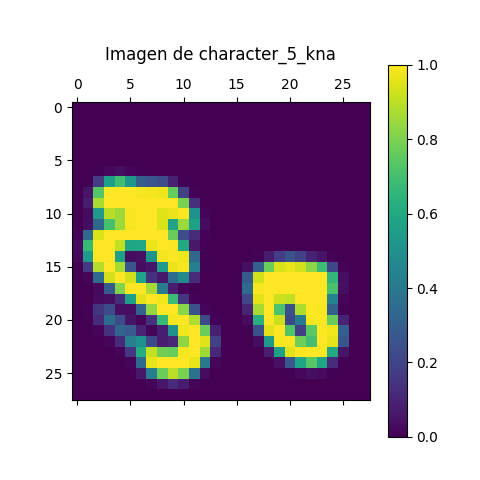
\includegraphics[width=87mm]{imgs/sample-kna.png}}
  \subfigure[Thresholding y closing]{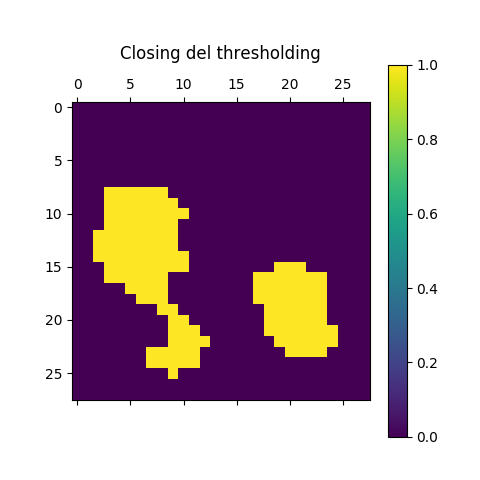
\includegraphics[width=87mm]{imgs/closing-thresholding.png}}
  \subfigure[Recortado de la caja englobante]{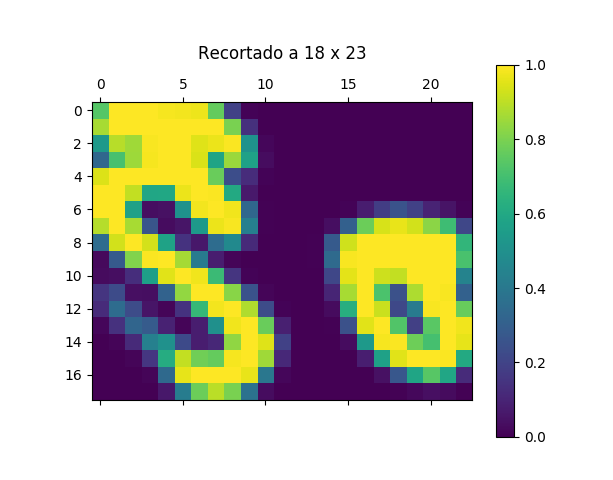
\includegraphics[width=87mm]{imgs/crop.png}}
  \subfigure[Reescalado]{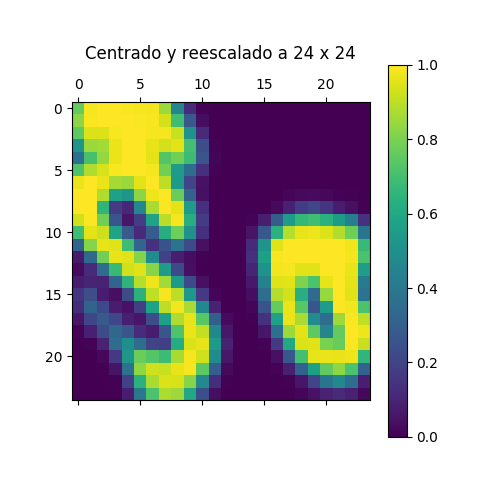
\includegraphics[width=87mm]{imgs/resize.png}}
  \caption{Proceso de centrado y reescalado sobre una instancia correspondiente al carácter kna}
  \label{fig:centerAndResize}
\end{figure}

\subsection{Downsampling}

Para reducir la dimensionalidad, realizamos un downsampling o
reducción por bloques de la imagen, agrupando cada bloque de 4
píxeles en uno usando la media de sus valores. Esta reducción se lleva
a cabo con la función \texttt{block\_reduce} de \textit{skimage}.

% Comentar que esta decisión es arriesgada y que nos hemos basado en
% validación con RF

\begin{figure}[H]
  \centering
  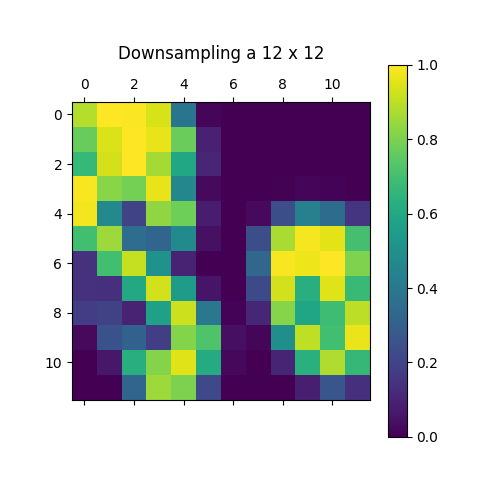
\includegraphics[width=87mm]{imgs/downsampling.png}
  \caption{Resultado del preprocesamiento (tras combinar centrado y reescalado con downsampling)}
  \label{fig:downsampling}
\end{figure}

\end{document}
